\documentclass[12pt, twoside]{article}
\usepackage[letterpaper, margin=1in, headsep=0.5in]{geometry}
\usepackage[english]{babel}
\usepackage[utf8]{inputenc}
\usepackage{amsmath}
\usepackage{amsfonts}
\usepackage{amssymb}
\usepackage{tikz}
\usetikzlibrary{quotes, angles}
\usepackage{graphicx}
\usepackage{enumitem}
\usepackage{multicol}
\usepackage{hyperref}

\newif\ifmeta
\metatrue %print standards and topics tags

\title{IB Mathematics}
\author{Chris Huson}
\date{January 2022}

\usepackage{fancyhdr}
\pagestyle{fancy}
\fancyhf{}
\renewcommand{\headrulewidth}{0pt} % disable the underline of the header
\raggedbottom


\fancyhead[LE]{\thepage}
\fancyhead[RO]{\thepage \\ Name: \hspace{4cm} \,\\}
\fancyhead[LO]{BECA / IB Math 03-Quadratic functions\\* 25 January 2022}

\begin{document}

\subsubsection*{4.2 Classwork: Cubic functions}
\begin{enumerate}
\item Part of the function $f(x)=x^3-5x^2+2x+8$ is shown on the graph.\\
    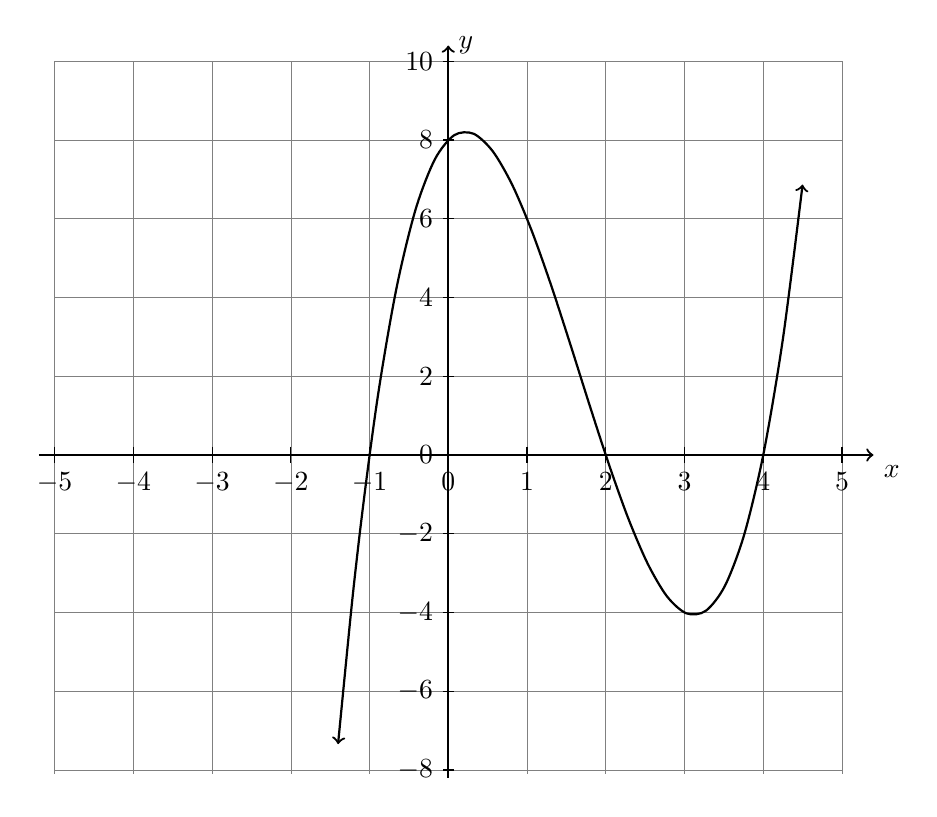
\begin{tikzpicture}[x=1cm, y=0.5cm]
        \draw [help lines] (-5,-8.1) grid (5,10);
        \draw [thick, ->] (-5.2,0) -- (5.4,0) node [below right] {$x$};
        \draw [thick, ->] (0,-8.2)--(0,10.4) node [right] {$y$};
        \foreach \x in {-5,...,5}
            \draw[shift={(\x,0)}] (0,3pt)--(0,-3pt) node[below] {$\x$};
        \foreach \y in {-8,-6,...,10}
            \draw[shift={(0,\y)}] (2pt,0pt)--(-2pt,0pt) node[left]  {$\y$};
        \draw [<->,thick,smooth,domain=-1.4:4.5] plot(\x,{(\x)^3-5*(\x)^2+2*(\x)+8});
    \end{tikzpicture}

    \begin{enumerate}
    \item Write down the $y$-intercept.
    \item Show that $f(0)$ is the $y$-intercept by substituting $x=0$ into the function $f(x)$.\vspace{1cm}
    \item Write down the $x$-intercepts.
    \item Show that $2$ is an $x$-intercept because $x=2$ is a solution to $f(x)=0$.\vspace{1cm}
    %\item What is the end behavior?
    %\begin{enumerate}
        %\item As $x\xrightarrow{}+\infty$ does $y\xrightarrow{}+\infty \text{ or } -\infty$?
        %\item As $x\xrightarrow{}-\infty$ does $y\xrightarrow{}+\infty \text{ or } -\infty$?
    %\end{enumerate}
    \item Label the local maximum and local minimum as ordered pairs (approximate the values).
    \item Slope: on the $x$-axis below, label the portion of the domain where $f$ is increasing with pluses (``+") and decreasing with negative signs (``-"). Mark the extrema (maximum and minimum) with zeros since $f(x)$ is horizontal at those points.
    \item Write down the intervals the function is increasing and decreasing.
    \end{enumerate}\vspace{1cm}
    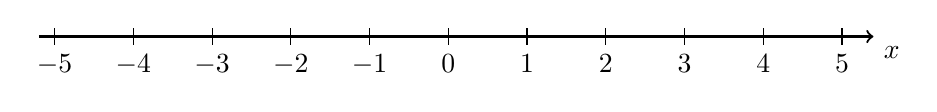
\begin{tikzpicture}[x=1cm]
        \draw [thick, ->] (-5.2,0) -- (5.4,0) node [below right] {$x$};
        \foreach \x in {-5,...,5}
            \draw[shift={(\x,0)}] (0,3pt)--(0,-3pt) node[below] {$\x$};
    \end{tikzpicture}

\newpage
\item The function $g(x)=-x^3-7x^2-14x-8$ is plotted below.\\
    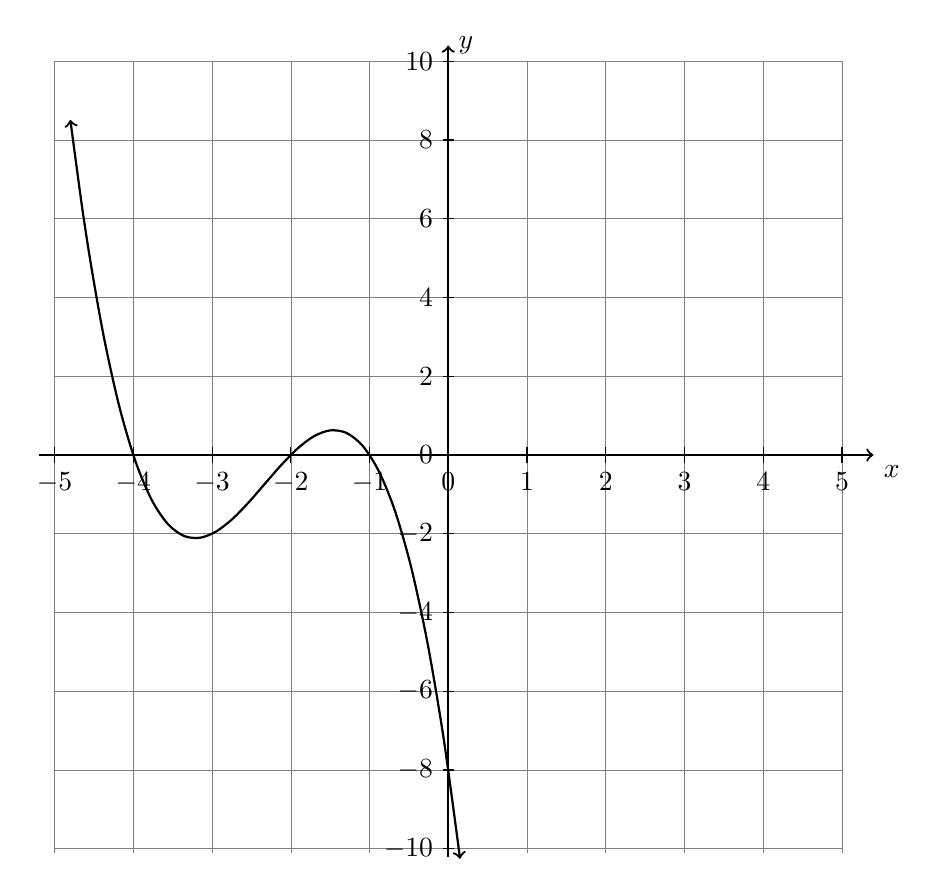
\begin{tikzpicture}[x=1cm, y=0.5cm]
        \draw [help lines] (-5,-10.1) grid (5,10);
        \draw [thick, ->] (-5.2,0) -- (5.4,0) node [below right] {$x$};
        \draw [thick, ->] (0,-10.2)--(0,10.4) node [right] {$y$};
        \foreach \x in {-5,...,5}
            \draw[shift={(\x,0)}] (0,3pt)--(0,-3pt) node[below] {$\x$};
        \foreach \y in {-10,-8,...,10}
            \draw[shift={(0,\y)}] (2pt,0pt)--(-2pt,0pt) node[left]  {$\y$};
        \draw [<->,thick,smooth,domain=-4.8:0.15] plot(\x,{-(\x)^3-7*(\x)^2-14*(\x)-8});
    \end{tikzpicture}

    \begin{enumerate}
    \item Write down the $y$-intercept.
    \item Show that $f(0)$ is the $y$-intercept by substituting $x=0$ into the function $f(x)$.\vspace{1cm}
    \item Write down the $x$-intercepts.
    \item Show that $-1$ is an $x$-intercept because $x=-1$ is a solution to $f(x)=0$.\vspace{1cm}
    %\item What is the end behavior?
    %\begin{enumerate}
        %\item As $x\xrightarrow{}+\infty$ does $y\xrightarrow{}+\infty \text{ or } -\infty$?
        %\item As $x\xrightarrow{}-\infty$ does $y\xrightarrow{}+\infty \text{ or } -\infty$?
    %\end{enumerate}
    \item Label the local maximum and local minimum as ordered pairs (approximate the values).
    \item Slope: on the $x$-axis below, label the portion of the domain where $f$ is increasing with pluses (``+") and decreasing with negative signs (``-"). Mark the extrema (maximum and minimum) with zeros since $f(x)$ is horizontal at those points.
    \item Write down the intervals the function is increasing and decreasing.
    \end{enumerate}\vspace{1cm}
    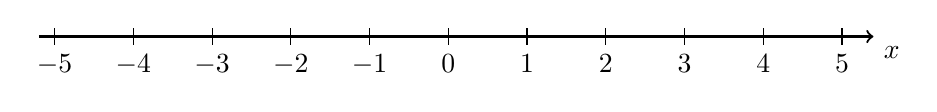
\begin{tikzpicture}[x=1cm]
        \draw [thick, ->] (-5.2,0) -- (5.4,0) node [below right] {$x$};
        \foreach \x in {-5,...,5}
            \draw[shift={(\x,0)}] (0,3pt)--(0,-3pt) node[below] {$\x$};
    \end{tikzpicture}

\newpage    
\item Given the function $h(x)=x^3+2x^2-5x-6$.
    \begin{enumerate}
        \item Write down the $y$-intercept. Mark it on the plot.
        \item Show that $-1$ is an $x$-intercept because $x=-1$ is a solution to $f(x)=0$. Mark $(-1, 0)$ on the graph as an $x$-intercept.\\*[20pt]
        \item The other $x$-intercepts are $-3$ and $+2$. Mark them on the plot.
    
        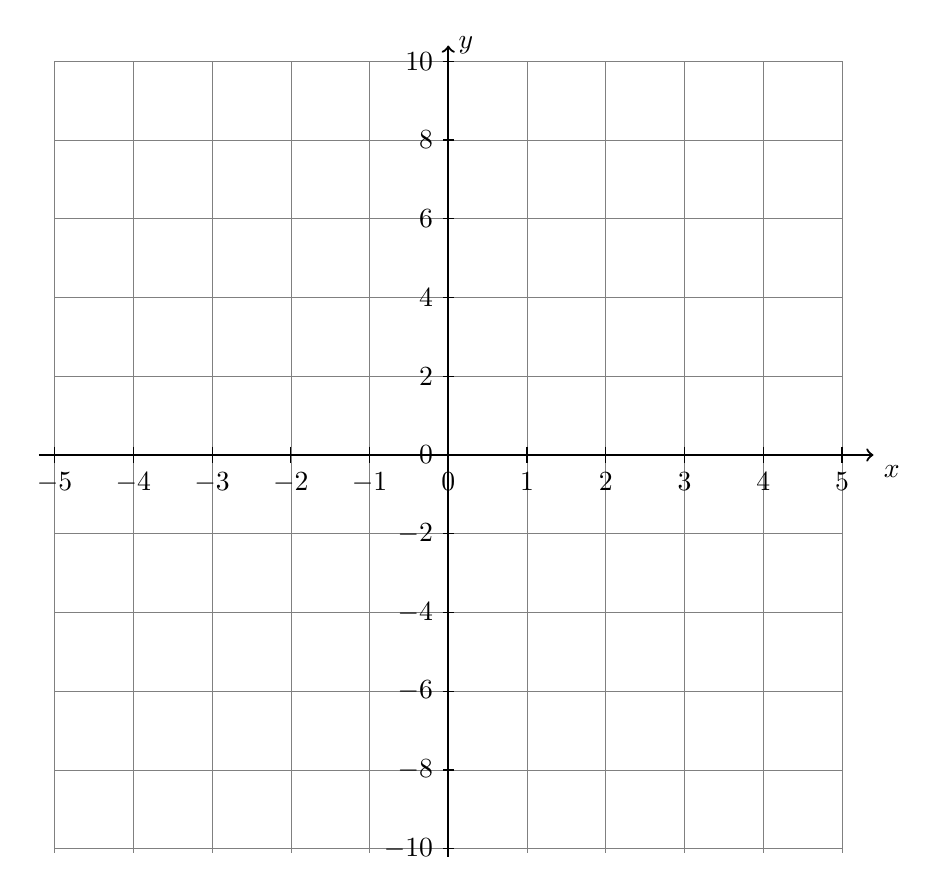
\begin{tikzpicture}[x=1cm, y=0.5cm]
            \draw [help lines] (-5,-10.1) grid (5,10);
            \draw [thick, ->] (-5.2,0) -- (5.4,0) node [below right] {$x$};
            \draw [thick, ->] (0,-10.2)--(0,10.4) node [right] {$y$};
            \foreach \x in {-5,...,5}
                \draw[shift={(\x,0)}] (0,3pt)--(0,-3pt) node[below] {$\x$};
            \foreach \y in {-10,-8,...,10}
                \draw[shift={(0,\y)}] (2pt,0pt)--(-2pt,0pt) node[left]  {$\y$};
            %\draw [<->,thick,smooth,domain=-4.8:0.15] plot(\x,{-(\x)^3-7*(\x)^2-14*(\x)-8});
        \end{tikzpicture}
    
        \item Graph the function on a calculator and, hence, sketch the curve.
    \end{enumerate}

\end{enumerate}
\end{document}



